\section{Introduction}\label{sec:intro}
Two-choice allocation assigns each item to the less loaded of two
candidates~\cite{azar}. We study the total number of items assigned beyond
bucket capacity. At total nominal capacity, overflow equals half the total
absolute deviation from capacity. Its prediction requires information beyond
the largest load.

We ask which information a reduced model must retain for two weakly coupled
communities. Each community has $q$ buckets with uniform internal bipartite
candidates. A fraction $\eps$ of candidates connect the communities through
any predetermined doubly stochastic kernel. Both fixed matchings and product
sampling have the required uniform endpoint marginals.
Ties favor the left endpoint, as in the internal two-group
Always-Go-Left rule of V\"ocking~\cite{vocking}.

With empty starts and integer capacity $c\asymp q$, critical fill occurs at
$n_*=2qc\asymp q^2$ arrivals. Without cross sampling, community choices
produce order-$q$ imbalance fluctuations. Cross arrivals can contribute order
$\eps q$ to the cumulative normalized drift. These scales motivate weak
coupling $\eps q\to\lambda<\infty$.

Every admissible fixed cross kernel has the same first-order critical law.
Internal load variation remains in that law, even at known community imbalance.
Expected overflow is order $q$, while its fraction of arrivals tends to zero.
Changing the fixed cross kernel preserves its leading coefficient.

Figure~\ref{fig:profileablation} shows the missing internal contribution.
Section~\ref{sec:experiments} separates this readout comparison from the
unconditional diffusion test.

\begin{figure}[t]
\centering
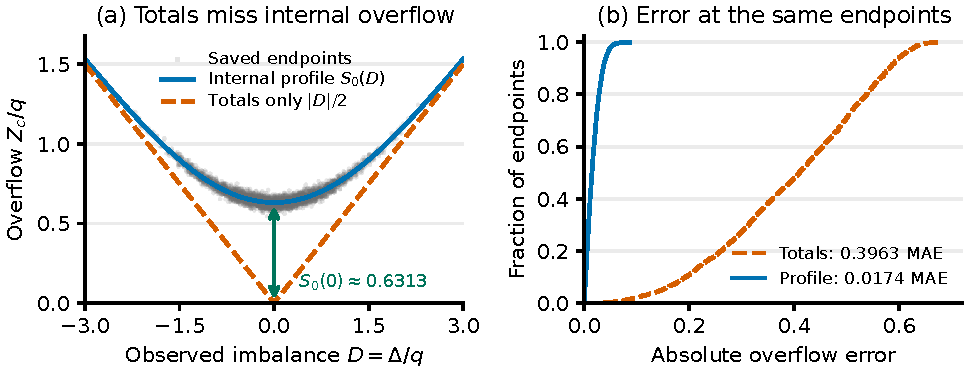
\includegraphics[width=\textwidth]{figures/readout_teaser.pdf}
\caption{Community totals miss internal overflow at critical fill.
Left: 4096 saved endpoints at $q=512$, $\kappa=1$, $\lambda=1$, with matching
crosses. The profile curve retains internal variation; $|D|/2$ uses only
community excess. Their gap at $D=0$ is approximately $0.6313$.
Right: absolute-error distributions for the same endpoints, with mean absolute
errors in the legend. Both readouts use the observed imbalance.
This is a descriptive mechanism comparison; the separate terminal test checks
the diffusion. The frozen profile lookup error is at most $0.000026$.}
\label{fig:profileablation}
\end{figure}

\subsection{Contributions}
Theorems~\ref{thm:universal}--\ref{thm:limit} establish three linked results.
\begin{enumerate}[label=(\roman*),leftmargin=*]
\item \textbf{Comparison of the actual allocation processes.}
For any predetermined doubly stochastic cross kernels, we couple the genuine
fixed-kernel process to the genuine product process. On each fixed $Tq^2$
horizon, their four sorted side vectors have expected uniform $\ell_1$
distance $O_{T,\Lambda}(q^{5/6}\log^2q)$ when $\eps q\le\Lambda$.
The bound controls imbalance and overflow at all common capacities.
Random-label forgetting first controls the whole cross load-pair table.
A coupling of sorted ranks then preserves the laws of both actual processes.
\item \textbf{An attracting internal lattice profile.}
We construct a unique mean-locked periodic family for the two-side tail flow.
It has full support, exponential moments, and uniform attraction on fixed
centered exponential-moment sublevels. An exact positive midpoint evolution
of signed tail differences gives strict contraction on equal-mean slices.
Its half-phase left/right identity records the asymmetric tie rule.
\item \textbf{A joint critical law for imbalance and overflow.}
For $\eps q\to\lambda$, normalized imbalance converges to a scalar diffusion.
Its restoring drift averages the fast common lattice phase.
The overflow curve retains the observation phase of the same internal profile.
Joint first Wasserstein convergence controls expected overflow as well as laws.
Corollaries~\ref{cor:internalexcess} and~\ref{cor:capacity} give the omitted
internal contribution and its capacity consequences.
\end{enumerate}
The capacity corollaries interpret the joint law for the fixed rule.

\subsection{Relation to previous work}
\textit{Existing rules and distribution equations.}
V\"ocking~\cite{vocking} introduced Always-Go-Left.
Berenbrink, Czumaj, Steger, and V\"ocking~\cite{bcsv} give sharp heavy-load
deviation bounds for greedy and asymmetric allocation.
Mitzenmacher~\cite{mitzode} uses differential equations to describe full load
distributions. We use this established distribution-level viewpoint.
The additional requirements here are long-time attraction of a two-type
integer-lattice profile and its coupling to a slow community imbalance.

\textit{Correlated choices and process comparison.}
Mitzenmacher~\cite{doublehash,doublecoupling} shows asymptotic equivalence
between double hashing and fully random balanced allocation, using fluid
limits and a coupling through a biased intermediate process.
The stated distribution results concern a constant number of choices and
$TN$ arrivals into $N$ bins for fixed $T$.
Our comparison treats arbitrary fixed doubly stochastic cross kernels,
allows only order-$q^{-1}$ cross probability, and covers $Tq^2$ arrivals.
It bounds the distance between the genuine fixed-kernel and product processes.
These differences are needed before passing to the critical overflow law.

\textit{Graphs and queues.}
Peres, Talwar, and Wieder~\cite{ptw} study graphical allocation and limited
choice. Bansal and Feldheim~\cite{bf} give a strategy based on graph
decompositions. Our rule compares only the two endpoint loads.
Queueing universality and diffusion limits~\cite{universality,bmw,atar}
include service and use different scales. Here each item has two candidates
and loads only increase.

\textit{Traveling profiles.}
Stolyar~\cite{stolyarwave,stolyarstationary} develops traveling-wave and
stationary-limit methods. Contraction and compactness are precedents.
The existence result in~\cite[Theorem 3]{stolyarwave} permits general jumps.
Its uniqueness and attraction result~\cite[Theorem 4]{stolyarwave} requires
a positive jump density bounded away from zero on compact subsets of
$\R_+$. The arithmetic-jump caveat following that theorem prevents its direct
use for the present lattice dynamics. We prove the two-side periodic-family
result directly, then obtain finite-system tracking without a stationary-limit
interchange. The later phase averaging acts on the slow drift, while the
critical overflow retains its endpoint phase.

Sections~\ref{sec:model}--\ref{sec:limit} state and prove the results.
Section~\ref{sec:experiments} evaluates their prediction steps.
The supplement gives numerical certificates, statistical protocols, and provenance.
